\begin{question}
    {5.8.6}
    {
        Let $b_0, b_1, b_2, \ldots$ be the sequence defined by the explicit formula
        \begin{equation*}
            b_n = C \cdot 3^n + D{(-2)}^n \quad \text{for all integers $n \geq 2$}
        \end{equation*}
        where $C$ and $D$ are real numbers. Show that for any choice of $C$ and $D$,
        \begin{equation*}
            b_k = b_{k-1} + 6b_{k-2} \quad \text{for all integers $k \geq 2$}
        \end{equation*}
        \vspace{-\baselineskip}
    }
\end{question}
\begin{proof}
    Let $b_0, b_1, b_2, \ldots$ be the sequence defined by the explicit formula
    \begin{equation*}
        b_n = C \cdot 3^n + D{(-2)}^n \quad \text{for all integers $n \geq 2$}
    \end{equation*}
    We must prove that $b_k$ is true when $b_n$ is plugged in with any choice of $C$ and $D$:
    \begin{align*}
        b_k &= b_{k - 1} + 6b_{k - 2} \\
            &= \left (C\cdot 3^{(k - 1)} + D(-2)^{(k - 1)} \right ) + 6 \left (C\cdot 3^{(k - 2)} + D(-2)^{(k - 2)} \right ) \\
            &= C\cdot 3^{(k - 1)} + D(-2)^{(k - 1)} + 6C\cdot 3^{(k - 2)} + 6D(-2)^{(k - 2)} \\
            &= C \left (3^{(k - 1)} + 2 \left (3^{(k - 1)} \right ) \right ) + D \left ((-2)^{(k - 1)} - 3(-2)^{(k - 1)} \right ) \\
            &= C \left (3 \left (3^{(k - 1)} \right ) \right ) + D \left (-2(-2)^{(k - 1)} \right ) \\
            &= C (3^k) + D(-2)^k \\
            &= b_k
    \end{align*}
    Thus, we have proved that, for any choice of $C$ and $D$,
    \begin{equation*}
        b_k = b_{k-1} + 6b_{k-2} \quad \text{for all integers $k \geq 2$}
    \end{equation*}
    \vspace{-\baselineskip}
\end{proof}

\begin{question}
    {5.8.9}
    {
        \begin{enumerate}
            \item[a.] Suppose a sequence of the form $1,t,t^2,t^3, \ldots, t^n \ldots$ where $t \neq 0$, satisfies the given recurrence relation (but not necessarily the initial conditions), and find all possible values of $t$.
            \item[b.] Suppose a sequence satisfies the given initial conditions as well as the recurrence relation, and find an explicit formula for the sequence.
        \end{enumerate}
        \begin{equation*}
            b_k = 7b_{k-1} - 10b_{k-2} \quad \text{for all integers $k \geq 2$}
        \end{equation*}
        \begin{equation*}
            b_0 = 2 \quad b_1=2
        \end{equation*}
        \vspace{-\baselineskip}
    }
\end{question}
\begin{proof}
    \begin{enumerate}
        \item[a.] 
            Suppose a sequence of the form $1,t,t^2,t^3, \ldots, t^n \ldots$ where $t \neq 0$, satisfies 
            \begin{equation*}
                b_k = 7b_{k-1} - 10b_{k-2} \quad \text{for all integers $k \geq 2$}
            \end{equation*}
            Since we suppose the sequence is of form $1, t, t^2, \ldots, t^n, \ldots$, by the characteristic equation of the second-order linear homogeneous recurrence relation with constant coefficients, 
            \begin{align*}
                t^2 - 7t + 10 &= 0 \\
                (t - 5)(t - 2) &= 0 \\
                t &= 2, 5
            \end{align*}
            Thus, the only possible values of $t$ are $2$ and $5$.
        \item[b.] 
            $b_0, b_1, b_2, \ldots$ satisfies the equation
            \begin{equation*}
                b_n = C\cdot 2^n + D\cdot 5^n \quad \text{for all integers $n \geq 0$}
            \end{equation*}
            for some constants $C$ and $D$ due to part (a) and the distinct roots theorem. We are given that $b_0 = 2, b_1 = 2$. Therefore, 
            \begin{align*}
                &\begin{cases} 
                    b_0 = C \cdot 2^0 + D \cdot 5^0 \\
                    b_1 = C \cdot 2^1 + D \cdot 5^1
                \end{cases}
                &\begin{cases} 
                    2 = C + D \\ 
                    2 = 2C + 5D
                \end{cases}
            \end{align*}
            Plugging in $C = 2 - D$, 
            \begin{align*}
                2(2 - D) + 5D &= 2 \\
                4 - 2D + 5D &= 2 \\
                4 + 3D &= 2 \\
                3D &= -2 \\
                D &= \dfrac{-2}{3}
            \end{align*}
            Thus,
            \begin{equation*}
                b_n = C\cdot 2^n + D\cdot 5^n \quad \text{for all integers $n \geq 0$}
            \end{equation*}
            \vspace{-\baselineskip}
            \begin{align*}
                C &= 2 - D \\
                D &= \dfrac{-2}{3} \\
                C &= \dfrac{8}{3}
            \end{align*}
            \vspace{-\baselineskip}
            \begin{equation*}
                b_n = \dfrac{8}{3}\cdot 2^n + \dfrac{-2}{3}\cdot 5^n \quad \text{for all integers $n \geq 0$}
            \end{equation*}
    \end{enumerate}
\end{proof}

\begin{question}
    {5.8.10}
    {
        \begin{enumerate}
            \item[a.] Suppose a sequence of the form $1,t,t^2,t^3, \ldots, t^n \ldots$ where $t \neq 0$, satisfies the given recurrence relation (but not necessarily the initial conditions), and find all possible values of $t$.
            \item[b.] Suppose a sequence satisfies the given initial conditions as well as the recurrence relation, and find an explicit formula for the sequence.
        \end{enumerate}
        \begin{equation*}
            c_k = c_{k-1} + 6c_{k-2} \quad \text{for all integers $k \geq 2$}
        \end{equation*}
        \begin{equation*}
            c_0 = 0 \quad c_1=3
        \end{equation*}
    }
\end{question}
\begin{proof}
    \begin{enumerate}
        \item[a.] 
            Suppose a sequence of the form $1,t,t^2,t^3, \ldots, t^n \ldots$ where $t \neq 0$, satisfies 
            \begin{equation*}
                c_k = c_{k-1} + 6c_{k-2} \quad \text{for all integers $k \geq 2$}
            \end{equation*}
            Since we suppose the sequence is of form $1, t, t^2, \ldots, t^n, \ldots$, by the characteristic equation of the second-order linear homogeneous recurrence relation with constant coefficients, 
            \begin{align*}
                t^2 - t - 6 &= 0 \\
                (t - 3)(t + 2) &= 0 \\
                t &= -2, 3
            \end{align*}
            Thus, the only possible values of $t$ are $-2$ and $3$.
        \item[b.] 
            $c_0, c_1, c_2, \ldots$ satisfies the equation
            \begin{equation*}
                c_n = C\cdot (-2)^n + D\cdot 3^n \quad \text{for all integers $n \geq 0$}
            \end{equation*}
            for some constants $C$ and $D$ due to part (a) and the distinct roots theorem. We are given that $c_0 = 0, c_1 = 3$. Therefore, 
            \begin{align*}
                &\begin{cases} 
                    c_0 = C\cdot (-2)^0 + D\cdot 3^0 \\
                    c_1 = C\cdot (-2)^1 + D\cdot 3^1
                \end{cases}
                &\begin{cases} 
                    0 = C + D \\
                    3 = -2C + 3D
                \end{cases}
            \end{align*}
            Plugging in $C = - D$, 
            \begin{align*}
                -2(-D) + 3D &= 3 \\
                2D + 3D &= 3 \\
                5D &= 3 \\
                D &= \dfrac{3}{5}
            \end{align*}
            Thus,
            \begin{equation*}
                c_n = C\cdot (-2)^n + D\cdot 3^n \quad \text{for all integers $n \geq 0$}
            \end{equation*}
            \vspace{-\baselineskip}
            \begin{align*}
                C &= - D \\
                D &= \dfrac{3}{5} \\
                C &= \dfrac{-3}{5}
            \end{align*}
            \vspace{-\baselineskip}
            \begin{equation*}
                c_n = \dfrac{-3}{5}\cdot (-2)^n + \dfrac{3}{5}\cdot 3^n \quad \text{for all integers $n \geq 0$}
            \end{equation*}
    \end{enumerate}
\end{proof}

\begin{question}
    {5.8.15}
    {
        Suppose a sequence satisfies the given recurrence relation and initial conditions. Find an explicit formula for the sequence.
        \begin{equation*}
            t_k = 6t_{k-1} - 9t_{k-2} \quad \text{for all integers $k \geq 2$}
        \end{equation*}
        \begin{equation*}
            t_0 = 1 \quad t_1=3
        \end{equation*}
    }
\end{question}
\begin{proof}
    Suppose a sequence of the form $t_0, t_1, t_2, \ldots$ satisfies 
    \begin{equation*}
        t_k = 6t_{k-1} - 9t_{k-2} \quad \text{for all integers $k \geq 2$}
    \end{equation*}
    Since we suppose the sequence is of form $t_0, t_1, t_2, \ldots$, by the characteristic equation of the second-order linear homogeneous recurrence relation with constant coefficients,
    \begin{align*}
        y^2 &- 6a + 9 = 0 \\
        y &= 3
    \end{align*}
    for some number $y$ that satisfies the Characteristic Equation. 
    Thus, the only possible value of $y$ is 3.
    Due to the single-root theorem, $t_0, t_1, t_2, \ldots$ satisfies the equation
    \begin{equation*}
        t_n = Cr^n + Dnr^n \quad \text{for all integers $n \geq 0$}
    \end{equation*}
    for some constants $C$ and $D$ and real root $r$.
    % Since $t_0 = 1, t_1 = 3$, then
    We are given that $t_0 = 1, t_1 = 3$. Therefore,
    \begin{align*}
        &\begin{cases}
            t_0 = C\cdot 3^0 + D(0)\cdot 3^0 \\
            c_1 = C\cdot 3^1 + D\cdot 3^1
        \end{cases}
        &\begin{cases} 
            1 = C \\ 
            3 = 3C + 3D
        \end{cases}
        &\begin{cases} 
            C = 1 \\ 
            D = 0
        \end{cases}
    \end{align*}
    Hence,
    \begin{equation*}
        t_n = 3^n \quad \text{for all integers $n \geq 0$}
    \end{equation*}
\end{proof}

\newpage
\begin{question}
    {5.8.24}
    {
        The numbers $\dfrac{1 + \sqrt{5}}{2}$ and $\dfrac{1 - \sqrt{5}}{2}$ that appear in the explicit formula for the Fibonacci sequence are related to a quantity called the \textit{golden ration} in Greek mathematics. Consider a rectangle of length $\phi$ units and height $1$, where $\phi > 1$.
        \begin{figure}[H]
            \centering
            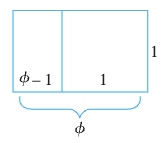
\includegraphics{5.8.24}
        \end{figure}
        Divide the rectangle into a rectangle and a square as shown in the preceding diagram. The square is $1$ unit on each side, and the rectangle has sides of length $1$ and $\phi - 1$.
        The ancient Greeks considered the outer rectangle to be perfectly proportioned (saying that the lengths of its sides were in a \textit{golden ratio} to each other) if the ratio of the length to the width of the outer rectangle equaled the ratio of the length to the width of the inner rectangle. That is,
        \begin{equation*}
            \frac{\phi}{1} = \frac{1}{\phi - 1}
        \end{equation*}
        \begin{enumerate}
            \item[a.] Show that $\phi$ satisfies the following quadratic equation $t^2 - t - 1 = 0$.
            \item[b.] Find the two solutions of $t^2 - t - 1 = 0$ and call them $\phi_1$ and $\phi_2$.
            \item[c.] Express the explicit formula for the Fibonacci sequence in terms of $\phi_1$ and $\phi_2$.
        \end{enumerate}
    }
\end{question}
\begin{proof}
    \begin{enumerate}
        \item[a.]
        \begin{align*}
            \frac{\phi}{1} &= \frac{1}{\phi - 1} \\
            \phi \cdot (\phi - 1) &= 1 \\
            \phi^2 - \phi &= 1 \\
            \phi^2 - \phi - 1 &= 0
        \end{align*}
        which is in the form $t^2 - t - 1 = 0$. Hence, $\phi$ satisfies the quadratic equation $t^2 - t - 1 = 0$.
        \item[b.]
        \begin{align*}
            \phi_1, \phi_2 &= \frac{-b \pm \sqrt{b^2 - 4ac}}{2a} \\
            &= \frac{1 \pm \sqrt{1 + 4}}{2} \\
            &= \frac{1 + \sqrt{1 + 4}}{2}, \frac{1 - \sqrt{1 + 4}}{2} \\
            &= \frac{1 + \sqrt{5}}{2}, \frac{1 - \sqrt{5}}{2} \\
            \phi_1 &= \frac{1 + \sqrt{5}}{2} \\
            \phi_2 &= \frac{1 - \sqrt{5}}{2}
        \end{align*}
        \item[c.] We know that the characteristic equation of the Fibonacci sequence has the solutions $\phi_1, \phi_2$. Due to the distinct-roots theorem, the Fibonacci sequence is given by the explicit formula:
        \begin{equation*}
            F_n = C\phi_1^n + D\phi_2^n \quad \text{for all integers $n \geq 0$}
        \end{equation*}
        for some constants $C$ and $D$. We are given that $F_0 = 0, F_1 = 1$. Therefore, when substituting for $n = 0, 1$ \\
        \begin{align*}
            \begin{cases}
                C + D = 1 \\ C\phi_1 + D\phi_2 = 1
            \end{cases}
        \end{align*}
        Plugging in $C = 1 - D$,
        \begin{align*}
            (1 - D)\phi_1 + D\phi_2 &= 1 \\
            D(\phi_2 - \phi_1) &= 1 - \phi_1 \\
            D &= \frac{1 - \phi_1}{\phi_2 - \phi_1}
        \end{align*}
        Thus,
        \begin{align*}
            C &= 1 - D \\
            C &= 1 - \frac{1 - \phi_1}{\phi_2 - \phi_1} \\
            C &= \frac{\phi_2 - \phi_1}{\phi_2 - \phi_1} - \frac{1 - \phi_1}{\phi_2 - \phi_1} \\
            C &= \frac{\phi_2 - 1}{\phi_2 - \phi_1}
        \end{align*}
        Therefore, the explicit formula for the Fibonacci Sequence in terms of $\phi_1$ and $\phi_2$ can be written as
        \begin{equation*}
            F_n = \dfrac{\phi_2 - 1}{\phi_2 - \phi_1}(\phi_1^n) + \dfrac{1 - \phi_1}{\phi_2 - \phi_1}(\phi_2^n) \quad \text{for all integers $n \geq 0$}
        \end{equation*}
    \end{enumerate}
\end{proof}